% Gerado automaticamente. No preambulo do documento use:
% \usepackage{pgfplots}
% \pgfplotsset{compat=1.18}
\definecolor{plotblue}{HTML}{2563EB}
\definecolor{plotorange}{HTML}{D97706}
\definecolor{plotgreen}{HTML}{059669}
\definecolor{plotpurple}{HTML}{7C3AED}
\definecolor{plotgray}{HTML}{374151}
\definecolor{plotred}{HTML}{DC2626}
\definecolor{plotteal}{HTML}{0F766E}
\definecolor{plotslate}{HTML}{64748B}

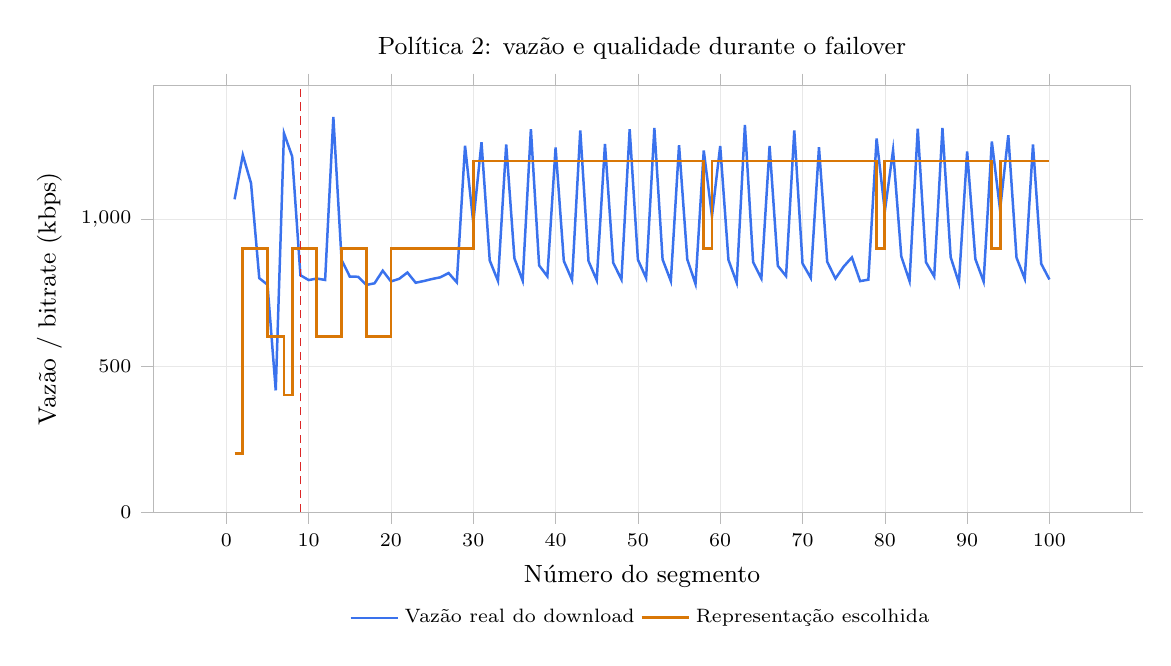
\begin{tikzpicture}
\begin{axis}[
    title={Política 2: vazão e qualidade durante o failover},
    xlabel={Número do segmento},
    ylabel={Vazão / bitrate (kbps)},
    width=14cm,
    height=7cm,
    grid=major,
    grid style={line width=.12pt, draw=gray!18},
    axis line style={draw=gray!55},
    tick style={draw=gray!55},
    tick align=outside,
    title style={font=\small},
    label style={font=\small},
    tick label style={font=\scriptsize},
    legend cell align={left},
    legend style={at={(0.5,-0.20)}, anchor=north, legend columns=3, draw=none, font=\scriptsize},
    ymin=0,
    ymax=1458.33
]
\addplot+[plotblue, line width=0.9pt, mark=none, opacity=0.9] coordinates {
(1,1069.05)
(2,1220.33)
(3,1123.9)
(4,799.51)
(5,777.1)
(6,415.8)
(7,1294.96)
(8,1215.36)
(9,809.51)
(10,793.01)
(11,798.13)
(12,793.38)
(13,1350.31)
(14,861.46)
(15,804.81)
(16,804.24)
(17,776.43)
(18,781.86)
(19,825.05)
(20,788.3)
(21,797.3)
(22,818.85)
(23,783.86)
(24,789.8)
(25,796.64)
(26,802.43)
(27,817)
(28,785.17)
(29,1252.22)
(30,989.53)
(31,1263.76)
(32,860.03)
(33,790.02)
(34,1256.66)
(35,867.19)
(36,791.1)
(37,1308.64)
(38,843.07)
(39,805.59)
(40,1245.93)
(41,858.4)
(42,793.08)
(43,1304.33)
(44,857.79)
(45,792.47)
(46,1258.27)
(47,852.28)
(48,794.87)
(49,1308.3)
(50,862.74)
(51,799.94)
(52,1313.17)
(53,863.38)
(54,789.77)
(55,1254.17)
(56,863.53)
(57,779.91)
(58,1235.87)
(59,1011.13)
(60,1251.17)
(61,862.23)
(62,784.3)
(63,1323.17)
(64,853.95)
(65,798.46)
(66,1250.98)
(67,841.63)
(68,806.46)
(69,1304.2)
(70,849.87)
(71,800.48)
(72,1246.8)
(73,855.29)
(74,798.18)
(75,839.03)
(76,870.45)
(77,789.35)
(78,794.32)
(79,1277.04)
(80,1028.31)
(81,1236.99)
(82,873.85)
(83,789.44)
(84,1310.59)
(85,853.98)
(86,805.24)
(87,1312.69)
(88,871.21)
(89,783.45)
(90,1232.25)
(91,864.86)
(92,788.16)
(93,1266.69)
(94,1033.07)
(95,1288.17)
(96,869.44)
(97,797.33)
(98,1256.49)
(99,848.77)
(100,794.96)
};
\addlegendentry{Vazão real do download}
\addplot+[plotorange, const plot, line width=1.05pt, mark=none] coordinates {
(1,200)
(2,900)
(3,900)
(4,900)
(5,600)
(6,600)
(7,400)
(8,900)
(9,900)
(10,900)
(11,600)
(12,600)
(13,600)
(14,900)
(15,900)
(16,900)
(17,600)
(18,600)
(19,600)
(20,900)
(21,900)
(22,900)
(23,900)
(24,900)
(25,900)
(26,900)
(27,900)
(28,900)
(29,900)
(30,1200)
(31,1200)
(32,1200)
(33,1200)
(34,1200)
(35,1200)
(36,1200)
(37,1200)
(38,1200)
(39,1200)
(40,1200)
(41,1200)
(42,1200)
(43,1200)
(44,1200)
(45,1200)
(46,1200)
(47,1200)
(48,1200)
(49,1200)
(50,1200)
(51,1200)
(52,1200)
(53,1200)
(54,1200)
(55,1200)
(56,1200)
(57,1200)
(58,900)
(59,1200)
(60,1200)
(61,1200)
(62,1200)
(63,1200)
(64,1200)
(65,1200)
(66,1200)
(67,1200)
(68,1200)
(69,1200)
(70,1200)
(71,1200)
(72,1200)
(73,1200)
(74,1200)
(75,1200)
(76,1200)
(77,1200)
(78,1200)
(79,900)
(80,1200)
(81,1200)
(82,1200)
(83,1200)
(84,1200)
(85,1200)
(86,1200)
(87,1200)
(88,1200)
(89,1200)
(90,1200)
(91,1200)
(92,1200)
(93,900)
(94,1200)
(95,1200)
(96,1200)
(97,1200)
(98,1200)
(99,1200)
(100,1200)
};
\addlegendentry{Representação escolhida}
\addplot+[plotred, line width=0.65pt, densely dashed, mark=none, forget plot] coordinates {(9,0) (9,1458.33)};
\end{axis}
\end{tikzpicture}
